\documentclass{standalone}

\usepackage[english]{babel}
\usepackage[linesnumbered, ruled, vlined]{algorithm2e}

\usepackage{caption}

% to create listings

\usepackage{listings, lstautogobble}
\lstset{
  autogobble=true,
  frame=single,
}

\lstdefinelanguage{coq}[Objective]{Caml}{
  morekeywords={Structure, Definition, Inductive, list, return},
  sensitive=true
}

% to define font size

\usepackage{ulem}
\usepackage{moresize}
\usepackage{anyfontsize}

% to use tikz and its libraries

\usepackage{tikz-timing}
\usepackage{tikz}

\usetikzlibrary{backgrounds}
\usetikzlibrary{positioning, calc, arrows, shapes, automata, petri, patterns}

% to use tikzmark, to place and refer to marks outside the current figure

\tikzset{every picture/.style={remember picture}}

% styles for transitions

\tikzset{transition/.append style={fill=black!20, thick}}
\tikzset{transition/.append style={fill=black!20, thick}}

% styles for test and inhib arcs.

\tikzstyle{test}=[pre, *-]
\tikzstyle{inhib}=[pre, o-]

% to use colors

\usepackage{xcolor}

%%%%%%%%%%%%%%%%%%%%%%%%%%%%%%%%%%%%%%%%%%%%%%%%%%
%                  BEGIN DOCUMENT                %
%%%%%%%%%%%%%%%%%%%%%%%%%%%%%%%%%%%%%%%%%%%%%%%%%%

\begin{document}

\begin{tikzpicture}

  \node (pn1) {
    \begin{tikzpicture}
      \node[place, tokens=1] (p0) [label={left:$p$}] {};
      \node[transition, anchor=north] (t0) at ($(p0.south)-(0,.5)$) {
      
      }
      edge[pre] (p0);

      \node[anchor=east] at ($(t0.west)$) {
        \begin{tabular}{@{}l@{}}
          $t$ \\
          \textcolor{red}{$c$} \\
        \end{tabular}
      };
      \node[anchor=west] at ($(t0.east)$) {
        \begin{tabular}{@{}l@{}}
          $[2,4]$ \\
          \textcolor{red}{${<}4{>}$} \\
        \end{tabular}
      };
      
    \end{tikzpicture}
  };

  \node (pn2) at ($(pn1.east)+(2,0)$) {
    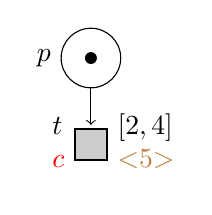
\begin{tikzpicture}
      \node[place, tokens=1] (p0) [label={left:$p$}] {};
      \node[transition, anchor=north] (t0) at ($(p0.south)-(0,.5)$) {
        
      }
      edge[pre] (p0);

      \node[anchor=east] at ($(t0.west)$) {
        \begin{tabular}{@{}l@{}}
          $t$ \\
          \textcolor{red}{$c$} \\
        \end{tabular}
      };
      \node[anchor=west] at ($(t0.east)$) {
        \begin{tabular}{@{}l@{}}
          $[2,4]$ \\
          \textcolor{brown}{${<}5{>}$} \\
        \end{tabular}
      };
      
    \end{tikzpicture}
  };

  \draw ($(pn1.east)-(.1,0)$) edge[->, double, line width=1pt] node[midway, above] {\Large$\downarrow$} ($(pn2.west)+(.1,0)$);
  
\end{tikzpicture}

\end{document}
%%% Local Variables:
%%% mode: latex
%%% TeX-master: t
%%% End:
